\documentclass[a4paper,12pt]{report}

% ------------------------
% Pacchetti di base
% ------------------------
\usepackage[utf8]{inputenc}
\usepackage[T1]{fontenc}
\usepackage[italian]{babel}
\usepackage{graphicx}
\usepackage{geometry}
\geometry{margin=3cm}
\usepackage{setspace}
\usepackage{amsfonts}
\onehalfspacing % interlinea 1.5

% ------------------------
% Inizio documento
% ------------------------
\begin{document}

% ------------------------
% Frontespizio
% ------------------------
\begin{titlepage}
    \centering
    
    % Logo in alto
    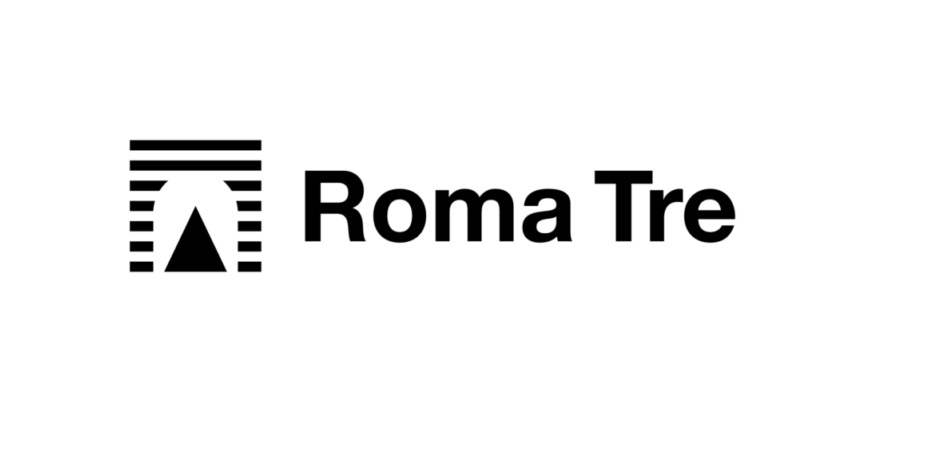
\includegraphics[width=6cm]{tesi/logo_uniroma3.jpeg}\par\vspace{0.5cm}
    
    {\large UNIVERSITÀ DEGLI STUDI ROMA TRE}\par
    \vspace{0.2cm}
    {\normalsize Dipartimento di Ingegneria Civile, Informatica e delle Tecnologie Aeronautiche}\par
    {\normalsize Corso di Laurea Triennale in Ingegneria Informatica}\par
    \vspace{1.5cm}
    
    {\large \textbf{Tesi di Laurea Triennale}}\par
    \vspace{1.5cm}
    
    {\Large \textbf{Sfruttare la fragility di un timetable \\ 
    per l'inserimento di un treno aggiuntivo \\ 
    in caso di eventi speciali}}\par
    \vspace{2cm}
    
    % Laureanda centrata
    \begin{center}
    \textbf{Laureanda} \\
    Alessia Ragheb \\
    Matricola 550427
    \end{center}
    
    \vspace{1.2cm}
    
    % Relatrice a sinistra
    \begin{flushleft}
    \textbf{Relatrice} \\
    Prof.ssa Marcella Samà
    \end{flushleft}
    
    \vfill
    
    {\normalsize Anno Accademico 2024/2025}\par
\end{titlepage}

% ------------------------
% Indice
% ------------------------
\tableofcontents

% ------------------------
% Introduzione (non numerata)
% ------------------------
\chapter*{Introduzione}
\addcontentsline{toc}{chapter}{Introduzione}

% Qui scrivi l’introduzione (3–4 pagine).
% Alla fine, quando sarà completa, fungerà da sintesi generale.

% ------------------------
% Capitolo 1
% ------------------------
\chapter{Stato dell’arte}
% → Qui inizia il primo capitolo numerato

\section{Evoluzione del trasporto ferroviario}

Il trasporto ferroviario da sempre costituisce una delle modalità più significative per lo spostamento di persone o merci. Nei primi tempi, quando le ferrovie erano ancora un fenomeno emergente e le corse erano poche e le infrastrutture ancora limitate : la pianificazione degli orari rimaneva uno strumento flessibile e poco complesso da gestire. Bastava quindi, in casi particolari e delicati, dare priorità a tratte a lunga percorrenza o ai treni merci più rilevanti, costruendo così di conseguenza il diagramma spazio-tempo su carta, dove i treni da gestire e coordinare venivano rappresentati con linee tracciate a mano. Questa pratica artigianale, che si basava dunque sull'esperienza e sull'intuizione dei tecnici, molto presto ha mostrato di avere i suoi limiti. Limiti emersi pian piano dalla sempre più crescente necessità di soddisfare un bisogno ovvero quello di trasportare in tempi sempre più ridotti, più persone o merci, sfruttando al massimo la capacità di un'infrastruttura e gestire quelli che possono essere possibili situazioni di conflitto fra treni.
Questo perchè uno dei limiti che comportava proprio questa pianificazione artigianale era la difficoltà di gestire possibili conflitti, simulare scenari alternativi o valutare l’impatto effettivo di un ritardo. 
La pianificazione degli orari non poteva più basarsi quindi sul vecchio metodo, impreciso e inaffidabile, ma iniziava a richiedere strumenti sempre più precisi in grado di garantire una buona affidabilità di tale servizio e questo per via delle nuove innovazioni avvenute negli decenni: come l'estensione delle linee a doppio binario, l'elettrificazione e l'introduzione di treni ad alta velocità, che hanno dunque contribuito ad arricchire sempre di più quella che è la complessità di una rete, diventa quindi impossibile gestire il tutto manualmente. La costruzione quindi di questi timetable divenne un vero e proprio problema di ottimizzazione, tanto da sviluppare modelli matematici e algoritmi in grado di gestire situazioni complicate e aumentare la robustezza di questa pianificazione, ciò ha trasformato l'orario nel vero cuore pulsante di un sistema ferroviario.
Per questo motivo, le compagnie ferroviarie investono mesi nella progettazione di un timetable, esaminando attentamente alcune soluzioni per soddisfare la domanda.



\subsection{Dall’artigianato all’ottimizzazione}
L’aumento della domanda e della densità dei treni ha trasformato la pianificazione degli orari, come abbiamo già detto, in un vero e proprio problema di ottimizzazione combinatoria. A partire dagli anni Settanta si sono diffusi i primi software per disegnare i diagrammi spazio–tempo, ma la logica di base rimaneva manuale. Con l’avvento dell’informatica e della ricerca operativa, il timetabling è stato formalizzato come un problema matematico con vincoli di capacità, precedenza e sicurezza. Algoritmi di programmazione lineare intera mista (MILP), tecniche di constraint programming ed euristiche sono stati sviluppati per generare orari efficienti e compatibili con i vincoli operativi.
Tuttavia, anche questi metodi tradizionali faticano a gestire reti sempre più congestionate: la presenza di molte variabili e vincoli rende proibitiva l’esplorazione dell’intero spazio delle soluzioni.



\subsection{Digitalizzazione e intelligenza artificiale}
Negli ultimi anni si è fatto un salto molto importante con l’adozione di strumenti basati su intelligenza artificiale (IA) e gemelli digitali. Le reti ferroviarie moderne generano enormi volumi di dati grazie a sensori distribuiti lungo l’infrastruttura e a bordo dei convogli. Algoritmi di machine learning utilizzano questi flussi per prevedere guasti e ottimizzare gli orari: un recente rapporto evidenzia che i modelli analizzano il flusso di passeggeri e i dati operativi per ridurre i ritardi e migliorare l’affidabilità.
Nel contempo, i gemelli digitali consentono di creare copie virtuali della rete, integrando sensori IoT, IA e cloud computing. Questi modelli simulano scenari come variazioni di domanda o condizioni meteorologiche, identificando la sequenza di tracce più efficiente e valutando l’effetto di modifiche operative.
Grazie alle simulazioni in tempo reale è possibile inserire margini di recupero mirati e prendere decisioni più veloci.
La digitalizzazione ha trasformato l’orario da documento statico a sistema “vivo” che si aggiorna continuamente. Mentre un tempo i timetables venivano rivisti poche volte l’anno, oggi i feed in tempo reale inviano aggiornamenti ogni pochi secondi e i sistemi AI monitorano lo stato della rete per intervenire prima che un piccolo ritardo si trasformi in un effetto domino.
I modelli predittivi hanno lo scopo di analizzare dati per suggerire interventi proattivi quali ricalcolare il percorso, ritardare un convoglio o avvisare i passeggeri di un cambio di binario.
Queste tecnologie sostengono la necessità di nuovi paradigmi per la pianificazione, basati su previsione, prevenzione e adattamento.


\subsection{Verso il quantum computing}
Negli ultimi anni si è iniziato a parlare anche di tecnologie più avanzate del solito, come il calcolo quantistico. L’idea è che questi nuovi strumenti possano aiutare a gestire situazioni molto complicate, come la costruzione appunto degli orari ferroviari, dove ci sono tantissime variabili da considerare. In questo senso, il calcolo quantistico viene visto come una possibile evoluzione naturale dopo i metodi classici e l’intelligenza artificiale, aprendo scenari interessanti per la pianificazione ferroviaria.
Questo approccio esplora un vasto spazio di soluzioni non raggiungibile dai metodi tradizionali, aprendo così una nuova frontiera per il timetabling.


\section{Cos’è un timetable e perché serve robusto}
Il timetable è, a tutti gli effetti, il piano che regola la circolazione ferroviaria. Non si tratta solo di indicare a che ora parte o arriva un treno: dentro ci sono i tempi di percorrenza, le precedenze da rispettare, le coincidenze che possono esserci. Sono dunque tutte informazioni necessarie a sfruttare la rete senza creare conflitti. 
È quindi la base organizzativa che permette di coordinare treni passeggeri o merci, garantendo che l’infrastruttura venga sfruttata al meglio delle sue possibilità e utilizzata in modo ordinato e sicuro.
Progettare un orario al giorno d'oggi significa però considerare molti fattori rispetto a un tempo: la domanda di mobilità, i vincoli di sicurezza, la disponibilità di personale e mezzi, i lavori di manutenzione e gli imprevisti come guasti o maltempo. Da queste scelte dipendono non solo i tempi di viaggio, ma anche aspetti organizzativi più ampi, come i turni del personale o l’uso del materiale rotabile.
Si parla di timetable robusto quando l’orario è costruito in modo da reggere a tutti gli effetti degli imprevisti. In una rete congestionata basta un piccolo ritardo per generare conseguenze a catena (i cosiddetti knock-on delays). Un orario robusto riesce ad assorbire questi ritardi primari, limitando la propagazione e mantenendo un servizio affidabile. Per questo spesso si inseriscono dei margini di recupero, detti buffer times, che permettono ai treni di rientrare più facilmente nei tempi previsti.
In sintesi, un timetable non è solo una tabella di orari: è l’ossatura del sistema ferroviario. E renderlo robusto significa assicurare che continui a funzionare in maniera stabile ed efficiente anche quando le condizioni non sono ideali.



\subsection{Perché servono orari robusti}
Un orario “perfetto sulla carta” non è sufficiente se non resiste agli imprevisti della realtà. Robustezza significa che l’orario può assorbire perturbazioni come ritardi, guasti o variazioni di domanda senza generare ritardi a cascata. Un orario per essere quindi robusto deve essere in grado di gestire sia le interruzioni programmate come la manutenzione, sia quelle non programmate, come un rallentamento o un ritardo alla partenza.
Per raggiungere questo obiettivo si introducono margini di recupero (buffer) tra i treni: più ampio è il buffer, maggiore è la perturbazione che l’orario può assorbire; tuttavia margini eccessivi riducono la capacità della rete. È quindi fondamentale trovare un compromesso tra efficienza e resilienza. \\ La robustezza viene spesso misurata in termini di disutilità totale: la somma ponderata del tempo di viaggio previsto e del ritardo medio. Orari con minore disutilità sono più robusti perché il ritardo medio che i passeggeri sperimentano risulta contenuto.
Gli studiosi suggeriscono di combinare simulazione e ottimizzazione esatta per generare orari robusti: la simulazione consente di valutare l’impatto delle perturbazioni mentre l’ottimizzazione trova la combinazione migliore di margini e sequenze.




\subsection{L’impatto della digitalizzazione sulla robustezza}
L’avvento dell’IA e dei gemelli digitali rende possibile valutare la robustezza in modo dinamico. Gli algoritmi di machine learning possono prevedere la propagazione di un ritardo attraverso la rete e suggerire modifiche in tempo reale, mentre le simulazioni basate su gemelli digitali permettono di testare diversi livelli di buffer e sequenze di tracce. 
Inoltre, i sistemi di analisi predittiva basati su big data aiutano a individuare i punti critici dell’orario e a rafforzarli prima che si verifichi un guasto.
La digitalizzazione, quindi, non solo migliora la pianificazione operativa ma offre anche strumenti per progettare orari più resilienti.
La robustezza non è un concetto assoluto ma uno spettro lungo il quale si misura la fragilità di un orario. Un orario fragile è molto sensibile a perturbazioni: un piccolo ritardo può generare un effetto domino di cancellazioni o perdite di coincidenza. Viceversa, un orario robusto può tollerare una certa quantità di imprevisti senza compromettere l’intero sistema. La distinzione tra robustezza e fragilità è fondamentale per comprendere dove e come intervenire nella pianificazione.


\subsection{Componenti della robustezza}
Quando si parla di robustezza di un timetable, non si intende una singola caratteristica, ma un insieme di elementi che concorrono a rendere l’orario sempre stabile. Le componenti principali possono essere così riassunte:

\begin{enumerate}

    \item \textbf{Margini temporali (buffer times)} \\
    Inserire piccole riserve di tempo tra un treno e l’altro consente di assorbire eventuali ritardi senza compromettere la regolarità del servizio. Questi margini, se ben distribuiti, permettono di recuperare deviazioni minori senza sacrificare troppa capacità della rete.

    \item \textbf{Tempo di riserva e recupero (recovery time)} \\
    Nei programmi di marcia è utile prevedere alcuni minuti in più rispetto al tempo minimo tecnico. Questa “scorta” può essere sfruttata per recuperare ritardi accumulati lungo la tratta, specialmente in prossimità delle stazioni principali o dei nodi più sensibili.

    \item \textbf{Capacità residua della rete} \\
    Un orario troppo saturo non lascia spazio a modifiche o recuperi. La robustezza dipende anche dal mantenere una certa quota di capacità non utilizzata, così da poter gestire deviazioni o inserire treni straordinari senza bloccare la circolazione.

    \item \textbf{Gestione dei conflitti} \\
    La robustezza non riguarda solo il singolo treno, ma anche il modo in cui più convogli interagiscono fra loro. Ridurre le situazioni di conflitto (incroci su binario unico, precedenze troppo ravvicinate, coincidenze non realistiche) è fondamentale per evitare che un ritardo locale si propaghi a tutta la rete.

    \item \textbf{Flessibilità operativa} \\
    Un orario robusto non deve essere “rigido”, ma deve consentire agli operatori di adattarsi. Ciò significa prevedere alternative praticabili, come instradamenti secondari, possibilità di sorpasso o soluzioni di emergenza che aiutino a contenere gli effetti domino.

    \end{enumerate}
    
    In conclusione, la robustezza è il risultato di un bilanciamento tra diversi elementi: non basta inserire più tempo dappertutto, ma occorre trovare il giusto compromesso tra efficienza, capacità e affidabilità.



\section{Robustezza e fragilità}
Negli studi sulla progettazione ferroviaria si parla spesso di robustezza come misura globale della qualità di un orario: un orario robusto limita il ritardo medio e la propagazione dei ritardi. Tuttavia, queste misure complessive non indicano dove l’orario è più vulnerabile. Sapere che un timetable è poco robusto non aiuta a identificare la tratta o la stazione che causa il problema, né a capire quali interventi potrebbero renderlo più resiliente. \\ Per affrontare questa carenza è stato introdotto il concetto di fragilità. \\ La fragilità è un indicatore locale che misura quanto un ritardo primario su una determinata coppia “treno–risorsa” (ad esempio, un treno che entra in una stazione o percorre una tratta) può propagarsi nel sistema. \\

applico un ritardo primario unitario $\delta_{t,r} = 1$ alla coppia treno--risorsa $(t,r)$


\[F(t,r) = \mathbb{E} \left[ \sum_{t' \in T} \Delta_{t'} \;\middle|\; \delta_{t,r} = 1 \right]\] \\ 

dove:
\begin{itemize}

    \item $F(t,r)$ rappresenta la fragilità della coppia $(t,r)$, 
    
    \item $\Delta_{t'}$ è il ritardo accumulato dal treno $t'$ a seguito della perturbazione,
    
    \end{itemize}
    In altre parole, indica il “costo di recupero” atteso: se un treno subisce un ritardo di un minuto in un punto specifico, quante ripercussioni avrà sull’orario? Un valore di fragilità alto significa che quel segmento è un punto debole: un piccolo ritardo potrebbe generare ritardi a catena, nonostante gli interventi dei dispatcher per riorganizzare i treni.
    L’aspetto interessante della fragilità è la sua località: non viene calcolata sull’intero orario, ma su ogni singola coppia treno–risorsa. Questo permette di costruire una “mappa delle criticità” della rete, evidenziando le sezioni dove un ritardo è più pericoloso e quelle dove è relativamente innocuo. Una volta calcolate le fragilità di tutte le coppie, si può aggregarle per ottenere un indice complessivo di robustezza o, meglio ancora, usarle per decidere dove intervenire: \\

\begin{enumerate}
    \item \textbf{aggiungere margini di recupero nelle sezioni più fragili.}

    \item \textbf{programmare la manutenzione nelle tratte più delicate.}

    \item \textbf{orientare gli investimenti infrastrutturali verso le stazioni o le linee che ne hanno più bisogno.}
    
    \end{enumerate}
    
La fragilità, quindi, non sostituisce la robustezza ma la integra, offrendo uno strumento operativo che collega la teoria alla pratica quotidiana di chi gestisce e progetta gli orari.



\section{Inserimento di treni extra}
Le compagnie ferroviarie devono molto spesso affrontare situazioni in cui è necessario inserire treni aggiuntivi. Questo accade, ad esempio, quando si svolgono eventi speciali che generano picchi di domanda, durante periodi festivi, o quando occorre organizzare convogli merci straordinari. Inserire un nuovo treno in un orario già molto fitto è una sfida: occorre trovare uno slot in cui il convoglio non interferisca con gli altri, non superi la capacità delle linee e non causi ritardi a catena.

Tradizionalmente, l’inserimento di treni extra avveniva in modo euristico: si cercava un intervallo di tempo libero e, se necessario, si spostavano alcuni treni per fare spazio al nuovo convoglio. Tuttavia, questo approccio può generare conflitti e aumentare la fragilità dell’orario. Utilizzando la mappa di fragilità, invece, è possibile individuare le sezioni meno sensibili ai ritardi.
Questa idea rappresenta il filo conduttore della tesi: dimostrare che la fragilità non è solo un indicatore teorico ma un vero strumento di supporto decisionale, capace di guidare l’inserimento di treni extra in un orario reale senza comprometterne la qualità.

% ------------------------
% Capitolo 2
% ------------------------
\chapter{Formalizzazione del problema}

\section{Definizione del problema}
Il lavoro nasce dall’esigenza pratica di inserire un treno aggiuntivo in una rete che ha già un orario definito, senza dover riprogettare l’intero timetable. L’inserimento deve essere sicuro, fattibile e “leggero”: niente conflitti, rispetto dei vincoli (headway, capacità di stazioni e tratte, tempi tecnici di percorrenza), minimo impatto sui treni esistenti e basso rischio di generare ritardi a catena. In altre parole: trovare quando e dove il treno può passare, con orari concreti, e con quale livello di rischio per la stabilità dell’orario.


\subsection{Perché è considerato a tutti gli effetti un problema?}
Non è “solo” aggiungere un treno.
L’orario reale molto spesso è già saturo: singoli binari unici, incroci delicati, stazioni con capienza limitata, coincidenze da proteggere, finestre di manutenzione. Ogni treno in più interagisce con quelli già presenti: anticipi/ritardi locali possono spostare precedenze e creare punti di conflitto. Inoltre i piccoli scostamenti non sono indipendenti: un ritardo primario su un passaggio “sensibile” può propagarsi e coinvolgere molti convogli. Per questo l’inserimento “alla cieca” è rischioso.



\subsection{Perché va risolto?}
La domanda può cambiare: eventi speciali, picchi stagionali, merci urgenti. Poter accogliere capacità aggiuntiva senza compromettere l’orario di base è un vantaggio operativo e di servizio. Un metodo che identifica gli slot giusti (finestre temporali) e misura il rischio locale permette di sfruttare la rete in modo mirato, mantenendo affidabilità e qualità percepita dai passeggeri.
Lo spazio delle soluzioni è combinatorio: ogni scelta di orario per il treno aggiuntivo influenza più risorse (stazioni, tratte) e più treni, con vincoli che cambiano per direzione, tipo di linea (binario unico/doppio) e capacità locale. Inoltre la rete non è omogenea: esistono “colli di bottiglia” dove un minuto vale più che altrove. Servono quindi criteri locali per capire dove l’orario “cede” più facilmente.
Un inserimento mal posizionato si paga in puntualità, affidabilità e costi operativi.


\subsection{Colli di bottiglia della rete}
Un aspetto fondamentale da considerare è che la rete ferroviaria, come abbiamo detto, non è omogenea: accanto a sezioni dove la capacità è relativamente abbondante, esistono punti più delicati che si comportano come veri e propri colli di bottiglia.\\ Tra questi rientrano le Block Points (Bp).\\  Le Block Points, cioè quelle stazioni intermedie in cui la linea si restringe e la gestione del traffico diventa più rigida. 
Sono stazioni che hanno la funzione di delimitare i cosiddetti blocchi di circolazione.
Le Block Points hanno un ruolo cruciale perché spesso si trovano in corrispondenza di tratte a binario unico, dove due treni non possono circolare contemporaneamente nello stesso segmento. \\ In questi casi, anche un ritardo minimo può bloccare l’accesso all’intera sezione, propagandosi su più convogli.
Il loro scopo principale è quindi garantire la sicurezza della marcia dei treni e regolare il flusso nelle tratte più critiche, in queste casi, le Block Points fungono da punto di attesa o instradamento.\\
Per questo motivo, nel metodo proposto, le Block Points vengono trattate con regole più severe: l’inserimento di un treno aggiuntivo in corrispondenza di tali stazioni è vincolato a margini di sicurezza maggiori e a controlli più stringenti sulla compatibilità temporale.


\subsection{Cosa rende il problema difficile?}
\begin{itemize}
\item conflitti di traccia o di stazione (violazioni di headway/capacità);

\item ritardi a cascata su tratte già dense;

\item rottura di coincidenze e riorganizzazioni operative (sorpassi non previsti, resequencing forzato);

\item soppressioni parziali o riduzione dell’offerta nelle ore successive;

\item perdita di robustezza dell’orario (quel tratto diventa più vulnerabile per tutta la giornata).
\end{itemize}


\section{Scenario di ritardo primario (unitario)}
Per valutare la robustezza di un orario non basta considerare se i treni sono correttamente allocati “sulla carta”: occorre stimare come il sistema reagisce quando si verificano piccoli intralci. Un approccio molto diffuso è quello degli scenari di ritardo primario, in cui si introduce artificialmente un ritardo elementare su una risorsa e si osserva come esso si propaga.
Uno scenario di ritardo primario unitario consiste nell’applicare un ritardo minimo (ad esempio 1 minuto) a una specifica coppia treno–risorsa (dove la risorsa può essere una stazione o una tratta). 
L’ipotesi è semplice: “se questo treno arriva o parte con un minuto di ritardo in questo punto, che cosa succede al resto dell’orario?”.
Qui entra in gioco quella che è l'analisi sistematica: si ripete lo stesso esperimento su tutte le coppie treno–risorsa fino ad ottenere una visione completa della rete, evidenziando così “nodi fragili” e “nodi resilienti”.
Gli scenari di ritardo primario unitario sono la base sperimentale per passare da una misura astratta di robustezza a un indice locale di fragilità. Questo approccio ci permette di trasformare un problema complesso e globale in un’informazione utilizzabile dal nostro algoritmo: scegliere, tra le varie finestre temporali disponibili, quelle con impatto minimo in caso di perturbazioni.


\section{Finestre temporali e influenze}

Quando si parla di inserire un treno aggiuntivo in un orario ferroviario, non si ragiona più soltanto in termini di “tracce già esistenti”, ma è necessario costruire una visione a intervalli temporali. 
L’idea è quella di dividere l’intero orizzonte temporale della giornata (ad esempio le 24 ore di esercizio) in finestre, cioè segmenti di tempo che rappresentano le opportunità reali o potenziali per collocare un nuovo treno. 
Una finestra temporale è dunque un intervallo di tempo caratterizzato dall'intervallo (start,end) durante il quale una determinata risorsa della rete (una stazione o una tratta) risulta disponibile, ossia non occupata da altri convogli. Ogni finestra può quindi essere vista come uno slot libero in cui inserire un treno senza violare i vincoli immediati di capacità.

Nel nostro modello, a ciascuna finestra vengono aggiunte ulteriori informazioni:

\begin{itemize}
 \item start: istante di inizio della disponibilità;


 \item end: istante di fine della disponibilità;

 \item fragilità: misura della fragilità associata a quell’intervallo, che rappresenta quanto un eventuale ritardo o modifica introdotto in quella finestra rischi di propagarsi;

 \item centro: il baricentro temporale dell’intervallo, utile per confrontare la coerenza tra finestre consecutive;

 \item tipo: caratterizzato a sua volta da due tipi : \\
  Reale: slot temporale con il quale indichiamo effettivamente la presenza di un treno. \\
  Artificiale: slot temporale costruito invece nei gap liberi tra due treni consecutivi per rendere esplicita la disponibilità in quel tratto.

\end{itemize} 
In questo senso, lo slot temporale non è soltanto un “vuoto” nel calendario, ma un intervallo caratterizzato da qualità (fragilità più o meno alta, maggiore o minore tolleranza agli imprevisti).
L’orizzonte temporale della rete viene dunque suddiviso in un insieme ordinato di finestre. 
Questa suddivisione avviene in due modi, finestre reali e finestre artificiali.
Il risultato è una griglia di slot che copre l’intera giornata, con lunghezze variabili e fragilità associate.



\subsection{Influenze e incastri}

Due finestre consecutive sono compatibili se:

\begin{itemize}
    \item rispettano la continuità temporale;


    \item hanno un centro temporale coerente (il centro della seconda è successivo a quello della prima);

    \item rispettano i vincoli di headway, direzione e capacità;

     \item non cadono in conflitto in punti sensibili come le Block Points.

  \end{itemize}
Le finestre temporali sono gli “slot” potenzialmente utilizzabili. \\ La divisione dell’orizzonte temporale in finestre consente di descrivere la disponibilità di risorse durante l'arco di tutta la giornata. \\ 
Tuttavia, le finestre non possono essere considerate in isolamento. È la loro sequenza coerente a determinare la possibilità effettiva di inserire un nuovo servizio. Per questo motivo introduciamo il concetto di influenza: ogni finestra condiziona la successiva, nel senso che ne restringe o amplia la fattibilità. Questo legame è ciò che consente di costruire un percorso fluido lungo più stazioni. \\ Le influenze tra finestre determinano dunque quali sequenze sono effettivamente percorribili, e quindi quale percorso ottimale è costruibile per il treno aggiuntivo.


\section{Metodo proposto}
Per affrontare il problema dell’inserimento di un treno aggiuntivo in un orario già esistente, ho deciso di sfruttare il concetto di fragilità come guida principale. \\ In questo modo, non solo individuiamo le finestre temporali disponibili, ma le valutiamo in base alla loro capacità di assorbire perturbazioni senza generare ritardi a catena.
Le finestre rappresentano la materia prima su cui l’algoritmo lavora. \\ Inserire un treno significa scegliere una sequenza di finestre compatibili tra loro (una per ogni risorsa del percorso) e incastrarle in modo fluido.
In pratica, il procedimento consiste nel calcolare la fragilità per ogni tratto, selezionare le sezioni con valori più bassi e verificare se un nuovo treno può essere inserito in quelle finestre senza creare conflitti. Questa idea rappresenta il filo conduttore della tesi: dimostrare che la fragilità non è solo un indicatore teorico ma un vero strumento di supporto decisionale, capace di guidare l’inserimento di treni extra in un orario reale senza comprometterne la qualità.
 Utilizzando la mappa di fragilità, è possibile individuare le sezioni meno sensibili ai ritardi: queste “finestre a bassa fragilità” sono gli slot ideali per inserire un treno aggiuntivo con il minimo impatto. 

 
 \subsection{Fattori aggiuntivi per la robustezza}
Oltre ai vincoli strettamente tecnici, il metodo proposto ha richiesto l’integrazione di altri elementi che servono a rafforzare la robustezza del percorso individuato:
\begin{itemize}
    \item Gestione delle sovrapposizioni: è stato necessario definire quanto due finestre potessero sovrapporsi, distinguendo tra casi tollerabili e casi da scartare.

   \item Compatibilità temporale: introdurre controlli sulla progressione del “centro” delle finestre, per assicurare che il percorso sia sempre crescente nel tempo.

  \item Capacità residua: valutare che l’inserimento non saturi completamente l’infrastruttura, lasciando comunque margini per eventuali recuperi o inserimenti futuri.

  \item Classificazione della fragilità: distinguere le finestre in fasce (ottime, buone, moderate, pericolose, critiche) per avere un quadro più dettagliato delle opportunità.

  \item Influenza tra treni: considerare le interazioni tra convogli, così che l’inserimento di uno non generi effetti negativi su altri già programmati.
  \end{itemize}
Questi accorgimenti hanno permesso di rendere il metodo più flessibile e aderente alla realtà, garantendo che la soluzione proposta non fosse solo valida “sulla carta”, ma che potrebbe essere applicabile anche in una rete reale.

\subsection{Vincoli e controlli necessari}
Per poter trasformare la teoria in un metodo applicabile, non è bastato ragionare in termini di fragilità e finestre. È stato necessario introdurre una serie di vincoli operativi e controlli aggiuntivi che riflettono le reali condizioni di una rete ferroviaria:
\begin{itemize}

\item Headway minimo: garantire una distanza temporale di sicurezza tra due treni consecutivi, per evitare conflitti e sovrapposizioni.

\item Tempi di percorrenza: rispettare i travel time tecnici tra una stazione e l’altra, senza soluzioni di continuità o anticipi impossibili.

\item Attese massime: limitare il tempo di permanenza in una stazione, per evitare che il nuovo treno rimanga fermo troppo a lungo generando inefficienze.

\item Direzione di marcia: mantenere coerenza tra salita e discesa, evitando situazioni in cui un treno risulterebbe incompatibile con il verso di percorrenza della linea.

\item Gestione delle Block Points: trattare con maggiore severità le sezioni più critiche della rete, dove la capacità è ridotta e i margini di errore sono minimi.

\end{itemize}
Questi vincoli non hanno lo scopo di complicare il problema, ma di garantire che l’inserimento sia realistico e sostenibile in un contesto operativo.





% ------------------------
% Capitolo 3
% ------------------------
\chapter{Metodologia e implementazione}
\section{Struttura dell’algoritmo}
\section{Classi e funzioni principali}
\section{Modulo di ottimizzazione}
\section{Gestione delle finestre di influenza}

% ------------------------
% Capitolo 4
% ------------------------
\chapter{Risultati e analisi}
\section{Dati di test}
\section{Verifica del metodo}
\section{Analisi degli scenari}
\section{Confronto con approccio globale}

% ------------------------
% Capitolo 5
% ------------------------
\chapter{Conclusioni e sviluppi futuri}
\section{Sintesi dei risultati}
\section{Vantaggi dell’approccio}
\section{Limiti e difficoltà}
\section{Sviluppi futuri}

% ------------------------
% Fine documento
% ------------------------
\end{document}
